\documentclass[10pt]{beamer}\usepackage[]{graphicx}\usepackage[]{color}
%% maxwidth is the original width if it is less than linewidth
%% otherwise use linewidth (to make sure the graphics do not exceed the margin)
\makeatletter
\def\maxwidth{ %
  \ifdim\Gin@nat@width>\linewidth
    \linewidth
  \else
    \Gin@nat@width
  \fi
}
\makeatother

\definecolor{fgcolor}{rgb}{0.345, 0.345, 0.345}
\newcommand{\hlnum}[1]{\textcolor[rgb]{0.686,0.059,0.569}{#1}}%
\newcommand{\hlstr}[1]{\textcolor[rgb]{0.192,0.494,0.8}{#1}}%
\newcommand{\hlcom}[1]{\textcolor[rgb]{0.678,0.584,0.686}{\textit{#1}}}%
\newcommand{\hlopt}[1]{\textcolor[rgb]{0,0,0}{#1}}%
\newcommand{\hlstd}[1]{\textcolor[rgb]{0.345,0.345,0.345}{#1}}%
\newcommand{\hlkwa}[1]{\textcolor[rgb]{0.161,0.373,0.58}{\textbf{#1}}}%
\newcommand{\hlkwb}[1]{\textcolor[rgb]{0.69,0.353,0.396}{#1}}%
\newcommand{\hlkwc}[1]{\textcolor[rgb]{0.333,0.667,0.333}{#1}}%
\newcommand{\hlkwd}[1]{\textcolor[rgb]{0.737,0.353,0.396}{\textbf{#1}}}%

\usepackage{framed}
\makeatletter
\newenvironment{kframe}{%
 \def\at@end@of@kframe{}%
 \ifinner\ifhmode%
  \def\at@end@of@kframe{\end{minipage}}%
  \begin{minipage}{\columnwidth}%
 \fi\fi%
 \def\FrameCommand##1{\hskip\@totalleftmargin \hskip-\fboxsep
 \colorbox{shadecolor}{##1}\hskip-\fboxsep
     % There is no \\@totalrightmargin, so:
     \hskip-\linewidth \hskip-\@totalleftmargin \hskip\columnwidth}%
 \MakeFramed {\advance\hsize-\width
   \@totalleftmargin\z@ \linewidth\hsize
   \@setminipage}}%
 {\par\unskip\endMakeFramed%
 \at@end@of@kframe}
\makeatother

\definecolor{shadecolor}{rgb}{.97, .97, .97}
\definecolor{messagecolor}{rgb}{0, 0, 0}
\definecolor{warningcolor}{rgb}{1, 0, 1}
\definecolor{errorcolor}{rgb}{1, 0, 0}
\newenvironment{knitrout}{}{} % an empty environment to be redefined in TeX

\usepackage{alltt}

%\usetheme{metropolis}
\usetheme[progressbar=head]{metropolis}
\defaultfontfeatures{ Scale = MatchUppercase }
\defaultfontfeatures[\rmfamily]{ Scale = 1}
\usepackage{unicode-math}

\usepackage{framed}

\usepackage{tikz}
\usetikzlibrary{positioning,fit,arrows}

\tikzset{
 a/.style
  = {node distance=4em, text width=2.7em, minimum height=4em},
 b/.style
  = {rectangle, draw, fill=gray!10, node distance=4em, text width=6em,
     text centered, rounded corners, minimum height=4em, thick},
 c/.style
  = {circle, draw, dashed, fill=orange!10, inner sep = 0pt, node distance=5em, thick},
 d/.style
  = {rectangle, draw, dashed, fill=red!10, node distance=4em, text width=6em,
     text centered, rounded corners, minimum height=4em, thick},
 l/.style
  = {draw, -latex, thick},
 lr/.style
  = {draw, latex-latex, thick, red},
 lb/.style
  = {draw, -latex, thick, blue},
  lo/.style
  = {draw, -latex, thick, orange},
  lg/.style
  = {draw, -latex, thick, green},
  mylabel/.style
  ={text width=6.5em, text centered}
}

\usepackage{abbrev}

%\usepackage[style=authoryear-comp,firstinits,sortcites,maxcitenames=2,%
%    mincitenames=1,maxbibnames=10,minbibnames=10,uniquename=mininit,%
%    uniquelist=minyear,sortfirstinits=true]{biblatex}
%\usepackage[backend=biber,style=alphabetic]{biblatex}
\usepackage[style=authoryear-comp,firstinits,sortcites,maxcitenames=2,%
    mincitenames=1,maxbibnames=10,minbibnames=10,uniquename=mininit,%
    uniquelist=minyear,sortfirstinits=true]{biblatex}
\addbibresource{info4plants.bib}
%\renewcommand{\bibfont}{\small}
\IfFileExists{upquote.sty}{\usepackage{upquote}}{}
\begin{document}





\pgfdeclareimage[height=10ex]{SenPEP_large}{figures/senpep_logo}
\pgfdeclareimage[width=0.19\textwidth]{SenPEP}{figures/senpep_logo}
\pgfdeclareimage[width=0.19\textwidth]{HYflame}{figures/HY_biot_text}
\pgfdeclareimage[width=0.15\textwidth]{ViPS}{figures/senpep_logo}
\pgfdeclareimage[width=0.12\textwidth]{SMS}{figures/SMS}
\pgfdeclareimage[width=0.11\textwidth]{ESP}{figures/ESP}
\pgfdeclareimage[width=0.15\textwidth]{ViPS}{figures/vips-logo}
\pgfdeclareimage[width=0.15\textwidth]{AKA}{figures/aka_logo}

\title{Ultimate vs.\ proximate questions}
\subtitle{Can plants use UVB to predict the future?}
\author{Pedro J. Aphalo}
\date{UV4Plants, Pécs, May 2016}
\institute[Univ.\ of Helsinki]{Department of Biosciences, University of Helsinki \\[1ex] and \\[1ex] Viikki Plant Science Center, University of Helsinki\\[1ex] \href{http://blogs.helsinki.fi/senpep-blog/}{\pgfuseimage{SenPEP_large}} }


	\begin{frame}
		\maketitle
	\end{frame}

	\begin{frame}[c]
		\begin{center}
			\begin{small}
				\copyright 2016 by Pedro J. Aphalo\\
				Department of Biosciences, University of Helsinki, Finland.\\
				\textcolor{blue}{\url{http://blogs.helsinki.fi/senpep-blog/}}\\[2ex]
			\end{small}

			\begin{footnotesize}
				`Can plants use UV to predict the future?' slide presentation by Pedro J. Aphalo is licensed under a Creative Commons Attribution-ShareAlike 4.0 International License.\\[2ex]

			\end{footnotesize}

			
\includegraphics[width=6em]{figures/by-sa}
		\end{center}
	\end{frame}

	\begin{frame}
		\frametitle{Outline}
		\tableofcontents
	\end{frame}

\section{Background}

\begin{frame}[<+->]
  \frametitle{An evolutionary viewpoint}
  \begin{itemize}
    \item The focus of my presentation will be the sensory abilities of plants from an evolutionary and fitness perspective.
    \item Fitness represents an \emph{ultime cause} (a \emph{why} question).
    \item The physiological and/or molecular mechanisms are \emph{proximate causes} (\emph{how} questionss).
    \item In animal ecology sensory ecology is an important discipline.
    \item In the case of plants this approach has been rarely used\ldots
    \item \ldots based on the assumption that sensory capabilities and specially information processing are very limited in plants.
    \item Now we know that this assumption does not hold.
  \end{itemize}
\end{frame}


\begin{frame}[<+->]
  \frametitle{Forecasting: its relation to fitness}
  \begin{itemize}
    \item The discussion of the role ``future perception'' in fitness is current \autocite{Novoplansky2016a}.
    \item We depend on informally forecasting all sorts of events every minute while awake.
    \item Sometimes we do this consciously, but most of the time we are not aware of what our brain is doing.
    \item We use forecasts at very different time scales and to many different ends.
    \item If we use the abstraction of information, and for a moment forget about how its processing is implemented\ldots
    \item \ldots it is easy to imagine that every organism must have evolved the capacity to ``forecast'' future events important for fitness.
    \item How information is processed, ``the machinery used'', does not need to be the same as long the information is acquired, transmitted, stored and combined succesfully.
  \end{itemize}
\end{frame}

\begin{frame}[<+->]
  \frametitle{Can plants forecast? Preemptive acclimation}
   \begin{itemize}
    \item Several plant responses can be only explained from the evolutive/fitness
    point of view as being a `preparation' to tolerate or escape future stress events or
    take advantage of future favourable conditions.
    \begin{itemize}
    \item Preemptive shade avoidance as a response to reflected far-red light from neighbouring
    plants.
    \item Eavesdropping-on/communicating-with neighbours to preemptively acclimate/prepare
    for drought, herbivore attacks, even to synchronize flowering among individuals.
    \item Possibly (a hypothesis we are studying) preemptive acclimation to future soil
    drying in response to high ultraviolet-B irradiance.
 \end{itemize}
  \end{itemize}
\end{frame}

\section{Why sensory ecology?}

%\begin{frame}[<+->]
%\frametitle{Sensory ecology approach}
%\begin{enumerate}
%  \item Focus on the acquisition and use of information by organisms
%  \item Well developed discipline for animals
%  \item Less developed for plants
%  \item Why?
%  \item \ldots plants' behaviour is not easy for humans to observe (slow\ldots)
%  \item \ldots intellectually we find the idea of brainless organisms \emph{solving problems} and \emph{assessing risks} alien
%  \item In abstract terms of flow, exchange, storage and use of information the concept of \emph{organisms as problem solvers} makes a lot of sense for any organism\ldots
%\end{enumerate}
%\end{frame}

\begin{frame}[<+->]
\frametitle{What sensory ecology tells us}
\begin{enumerate}
  \item Information sources are crucial to the performance and survival of organims\ldots
  \item \ldots $\Rightarrow$ cross-correlations among variables in their environment and their lags, and autocorrelations, are key sources of information
  \item \ldots $\Rightarrow$ we need to pay attention to `joint statistical properties of environmental variables'\ldots
\end{enumerate}
\end{frame}

\begin{frame}
  \frametitle{Correlations in the environment}
  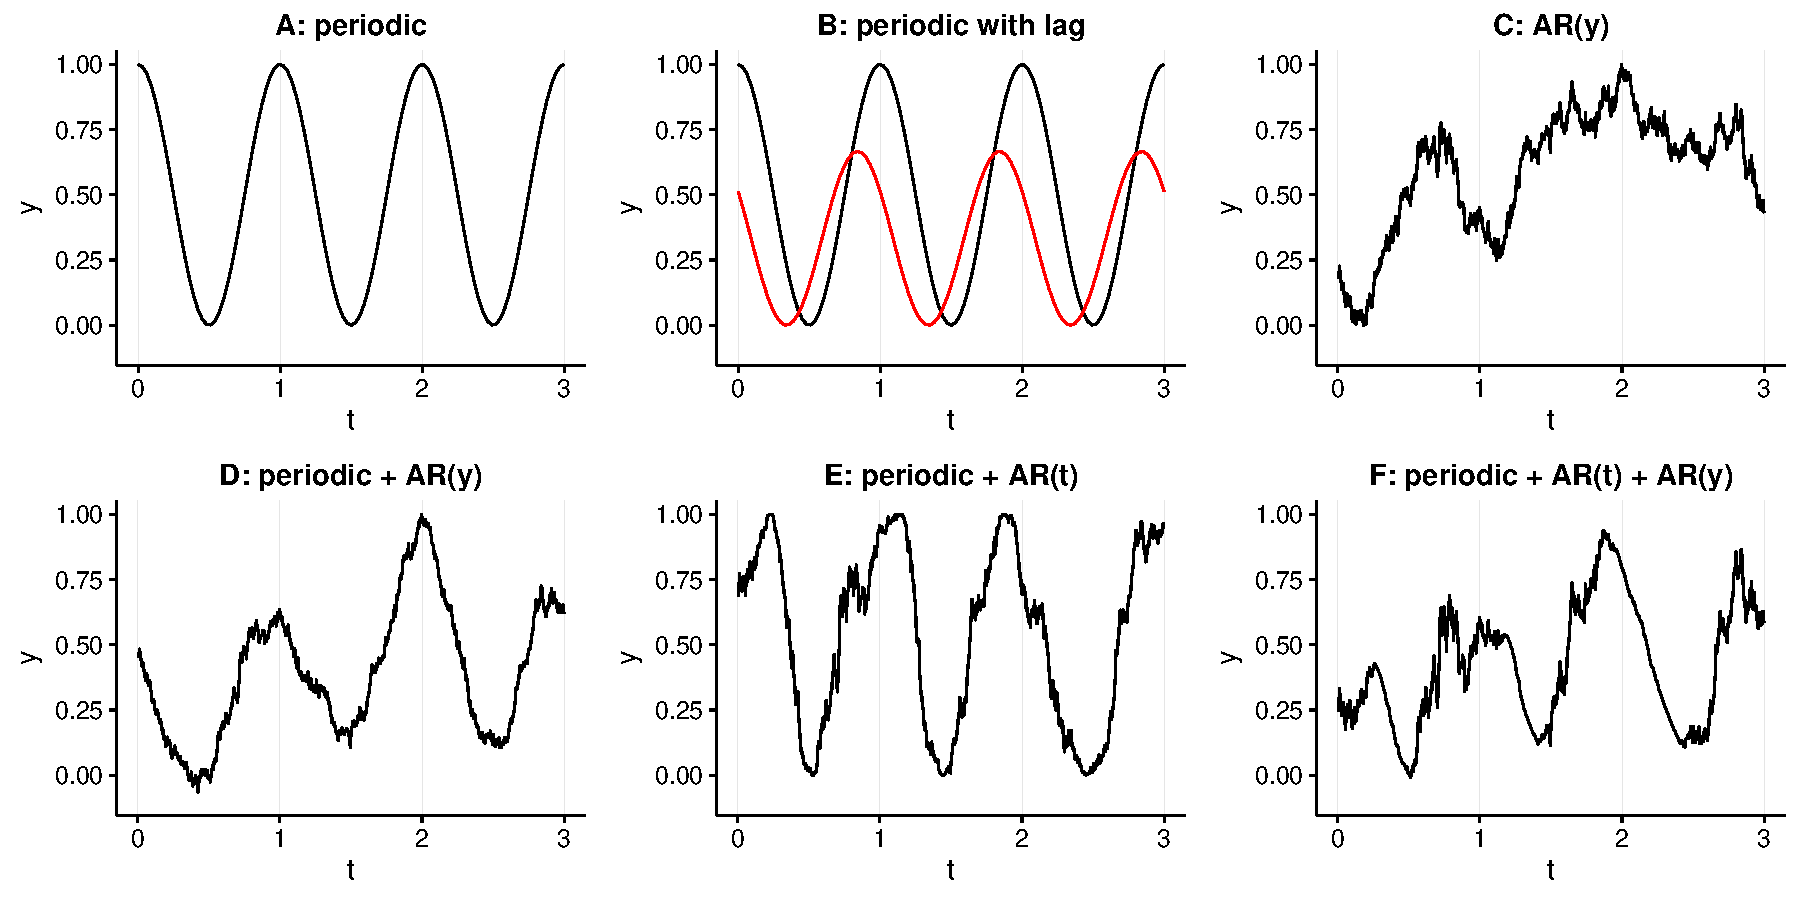
\includegraphics[width=\linewidth]{figures/cor_examples2.pdf}
\end{frame}

\section{A possible framework}


\begin{frame}{We propose a theoretical framework}

\begin{itemize}
\item<1-11>[]Conceptual framework\vspace{1ex}\pause

\centering
\tiny
  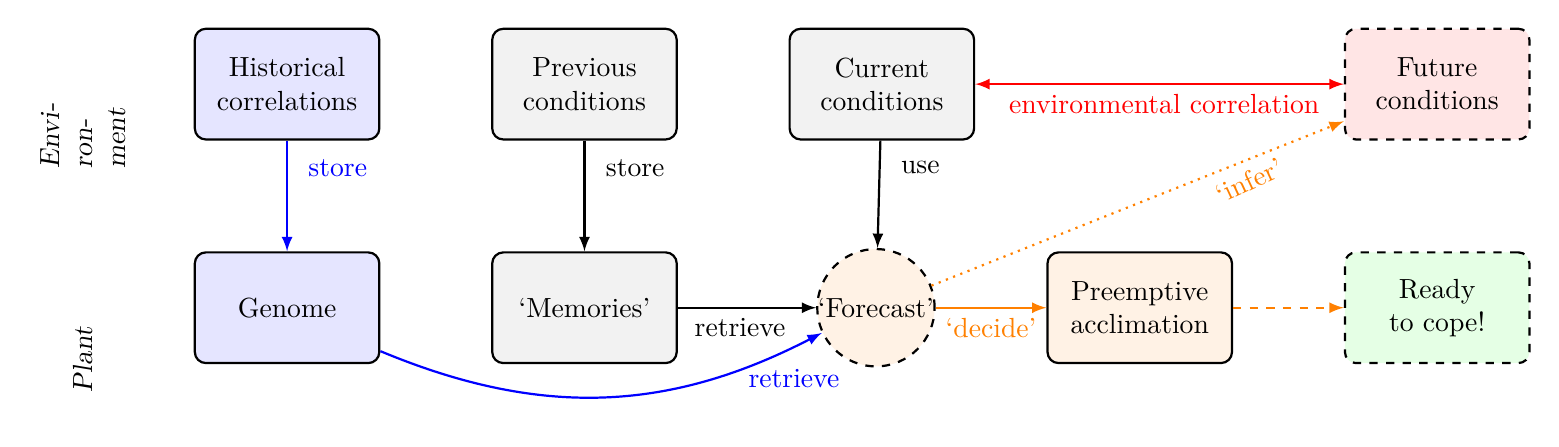
\begin{tikzpicture}[auto]
    \node [a, rotate=90] (environment) {\textsl{Environment}};
    \node [b, right = of environment, fill=blue!10] (history) {Historical correlations};
    \node [b, right = of history] (stress) {Previous conditions};
    \node [b, right = of stress] (data) {Current conditions};\pause
    \node [b, below = of stress] (memory) {`Memories'};
    \node [c, right = of memory] (info) {`Forecast'};
    \node [b, below = of history, fill=blue!10] (genome) {Genome};
    \node [a, rotate=90, left = of genome] (plant) {\textsl{Plant}};\pause
    \node [b, right = of info, fill=orange!10] (acclimation) {Preemptive acclimation};
    \node [d, right = of acclimation, fill=green!10] (ready) {Ready to cope!};
    \node [d, above = of ready] (stress2) {Future conditions};\pause

    \path [l] (stress) -- (memory) node[near start,right]{\hspace{0.4em}store};
    \path [lb] (history) -- (genome) node[near start, right]{\hspace{0.4em}store};\pause
    \path [l] (data) -- (info) node[near start,right]{\hspace{0.4em}use};
    \path [l] (memory) -- (info) node[near start,below]{\hspace{2em}retrieve};
    \path [lb] (genome) edge [bend right=25]  node[near end, right]{\hspace{1em}retrieve} (info);\pause
    \path [lr] (stress2) -- (data) node[near end,below]{\hspace{7em}environmental correlation};\pause
    \path [lo, dotted] (info) -- (stress2) node[near end,below,rotate=25]{`infer'};\pause
    \path [lo] (info) -- (acclimation) node[near start,below]{\hspace{2em}`decide'};\pause
\path [lo, dashed] (acclimation) -- (ready);

\end{tikzpicture}

\item<11-12>[]UVB example\vspace{1ex}\pause

\centering
\tiny
  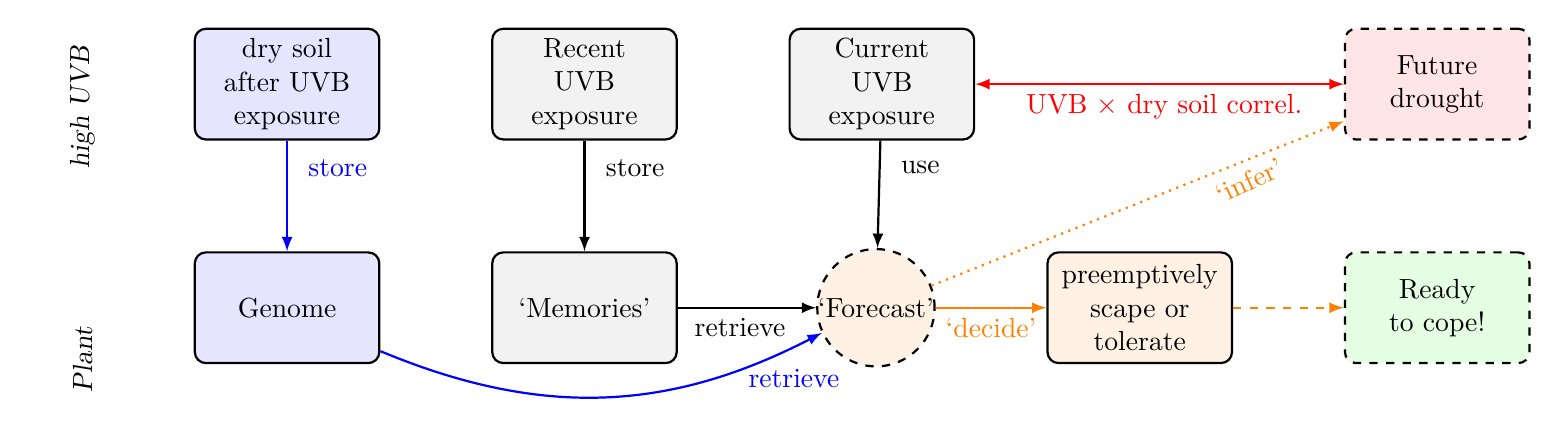
\begin{tikzpicture}[auto]
    \node [a, rotate=90] (environment) {\textsl{high~UVB}};
    \node [b, right = of environment, fill=blue!10] (history) {dry soil\\ after UVB\\ exposure};
    \node [b, below = of history, fill=blue!10] (genome) {Genome};
    \node [a, rotate=90, left = of genome] (plant) {\textsl{Plant}};
    \node [b, right = of history] (stress) {Recent\\ UVB\\ exposure};
    \node [b, right = of stress] (data) {Current\\ UVB\\ exposure};
    \node [b, below = of stress] (memory) {`Memories'};
    \node [c, right = of memory] (info) {`Forecast'};
    \node [b, right = of info, fill=orange!10] (acclimation) {preemptively scape or tolerate};
    \node [d, right = of acclimation, fill=green!10] (ready) {Ready to cope!};
    \node [d, above = of ready] (stress2) {Future drought};

    \path [l] (data) -- (info) node[near start,right]{\hspace{0.4em}use};
    \path [l] (memory) -- (info) node[near start,below]{\hspace{2em}retrieve};
    \path [l] (stress) -- (memory) node[near start,right]{\hspace{0.4em}store};
    \path [lb] (history) -- (genome) node[near start, right]{\hspace{0.4em}store};
    \path [lb] (genome) edge [bend right=25]  node[near end, right]{\hspace{1em}retrieve} (info);
    \path [lo] (info) -- (acclimation) node[near start,below]{\hspace{2em}`decide'};
     \path [lo, dotted] (info) -- (stress2) node[near end,below,rotate=25]{`infer'};
   \path [lr] (stress2) -- (data) node[near end,below]{\hspace{7em}UVB $\times$ dry soil correl.};
    \path [lo, dashed] (acclimation) -- (ready) node[near start,below]{};

\end{tikzpicture}

\end{itemize}
%%\vspace{-6ex}
%\caption{\footnotesize\sffamily Information use in preemptive acclimation to drought by perception of UV-B radiation. Arrows represent flows of information: \textcolor{blue}{\textbf{blue}} = retrieved from genome (stored during earlier generations), \textbf{black} = acquired and/or `memorized' during an individual's lifetime, \textcolor{red}{\textbf{red}} = lagged correlation between UV-B radiation and drought (e.g.\ low soil water content and high evaporative demand), \textcolor{orange}{\textbf{orange}} = represents the outcome of `data processing'. The outcome is a `decision' on how to adjust function, morphology and development to achieve drought tolerance based on an `implicit forecast of impending drought'. Time runs from left to right, with dashed boxes representing the future. `Conditions' refer to both external environment and plant's internal status.}\label{fig:drought:info}
\end{frame}

\section{Available evidence}

\begin{frame}
  \frametitle{Is there an environmental correlation? Yes}
  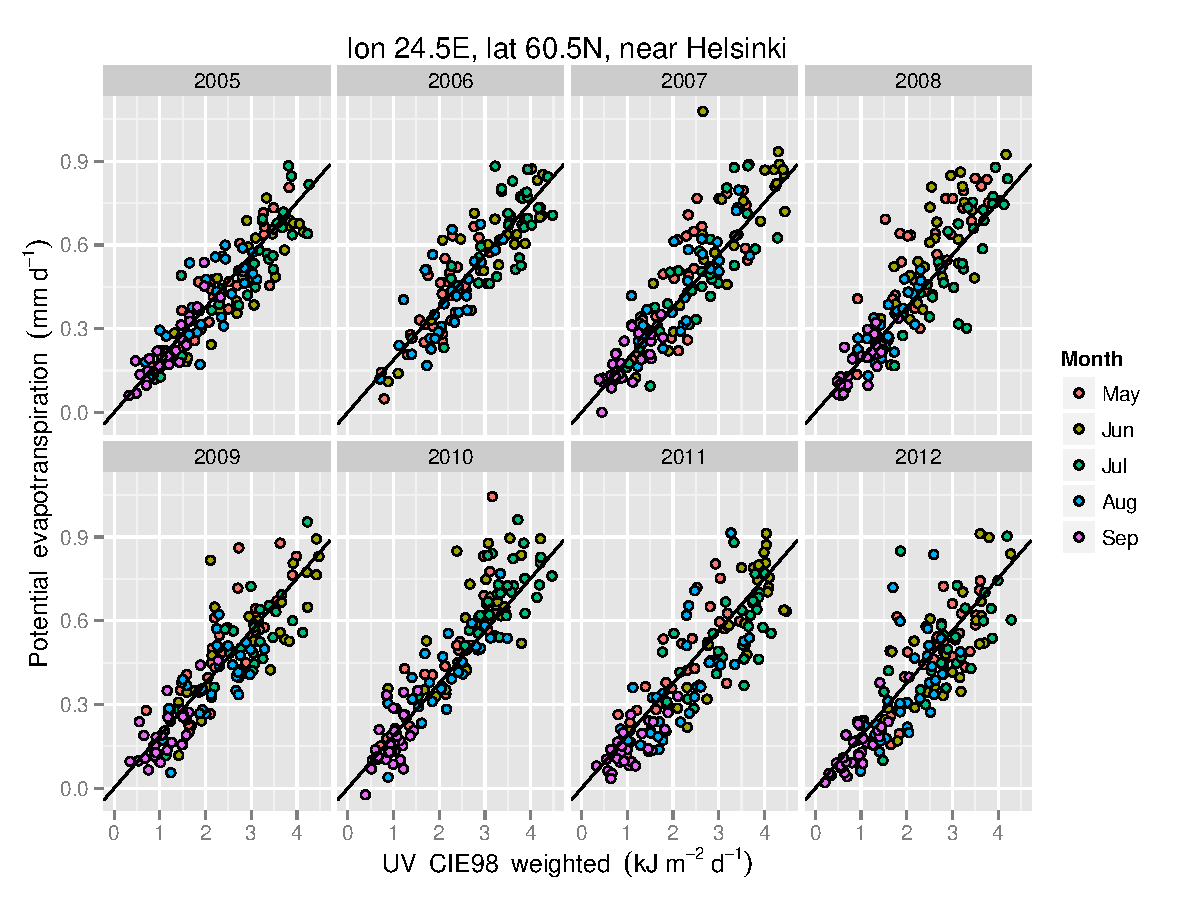
\includegraphics[width=0.8\linewidth]{figures/PET-CIE.pdf}

  (P. J. Aphalo, A. Lindfors, unpublished)
\end{frame}

\begin{frame}
  \frametitle{Is there an environmental correlation? Yes}
  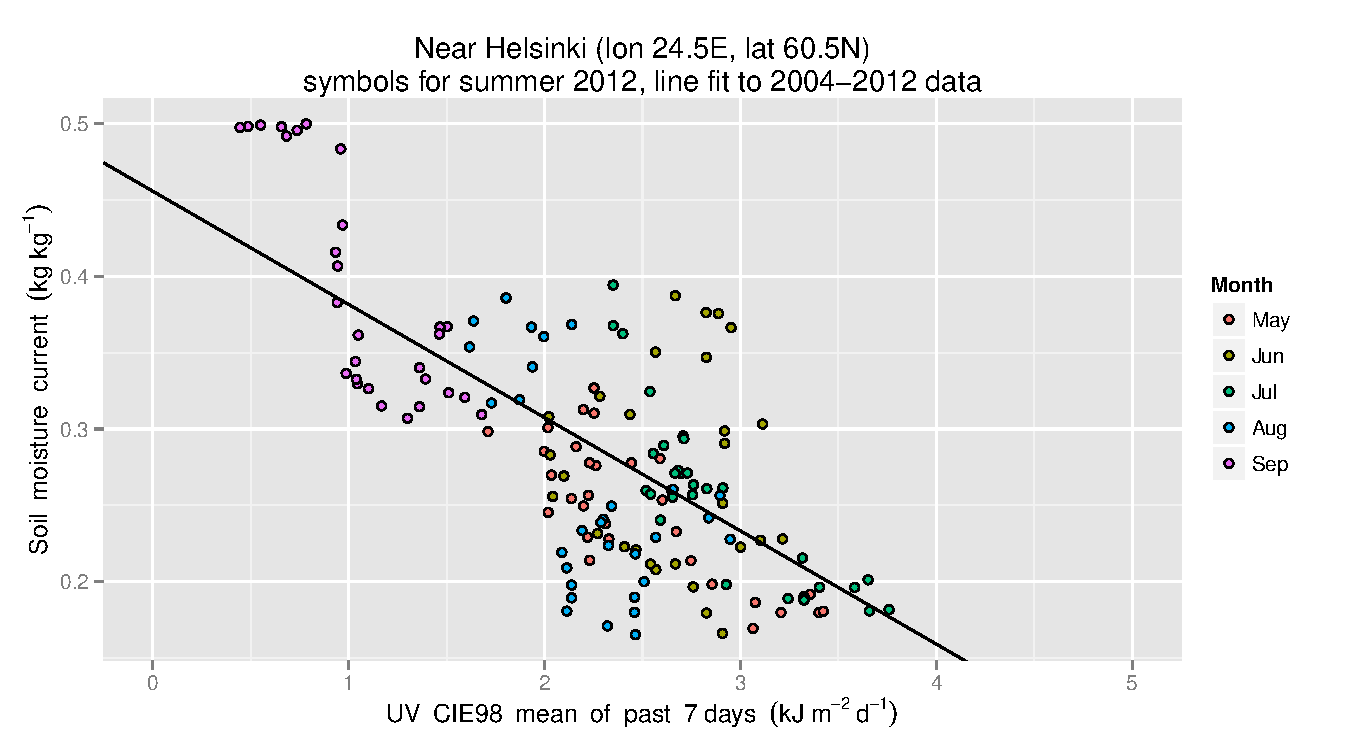
\includegraphics[width=\linewidth]{figures/soil-CIEmean.pdf}

  (P. J. Aphalo, A. Lindfors, unpublished)
\end{frame}

\begin{frame}
  \frametitle{Can exposure to UV-B trigger drought-acclimation? Yes}
  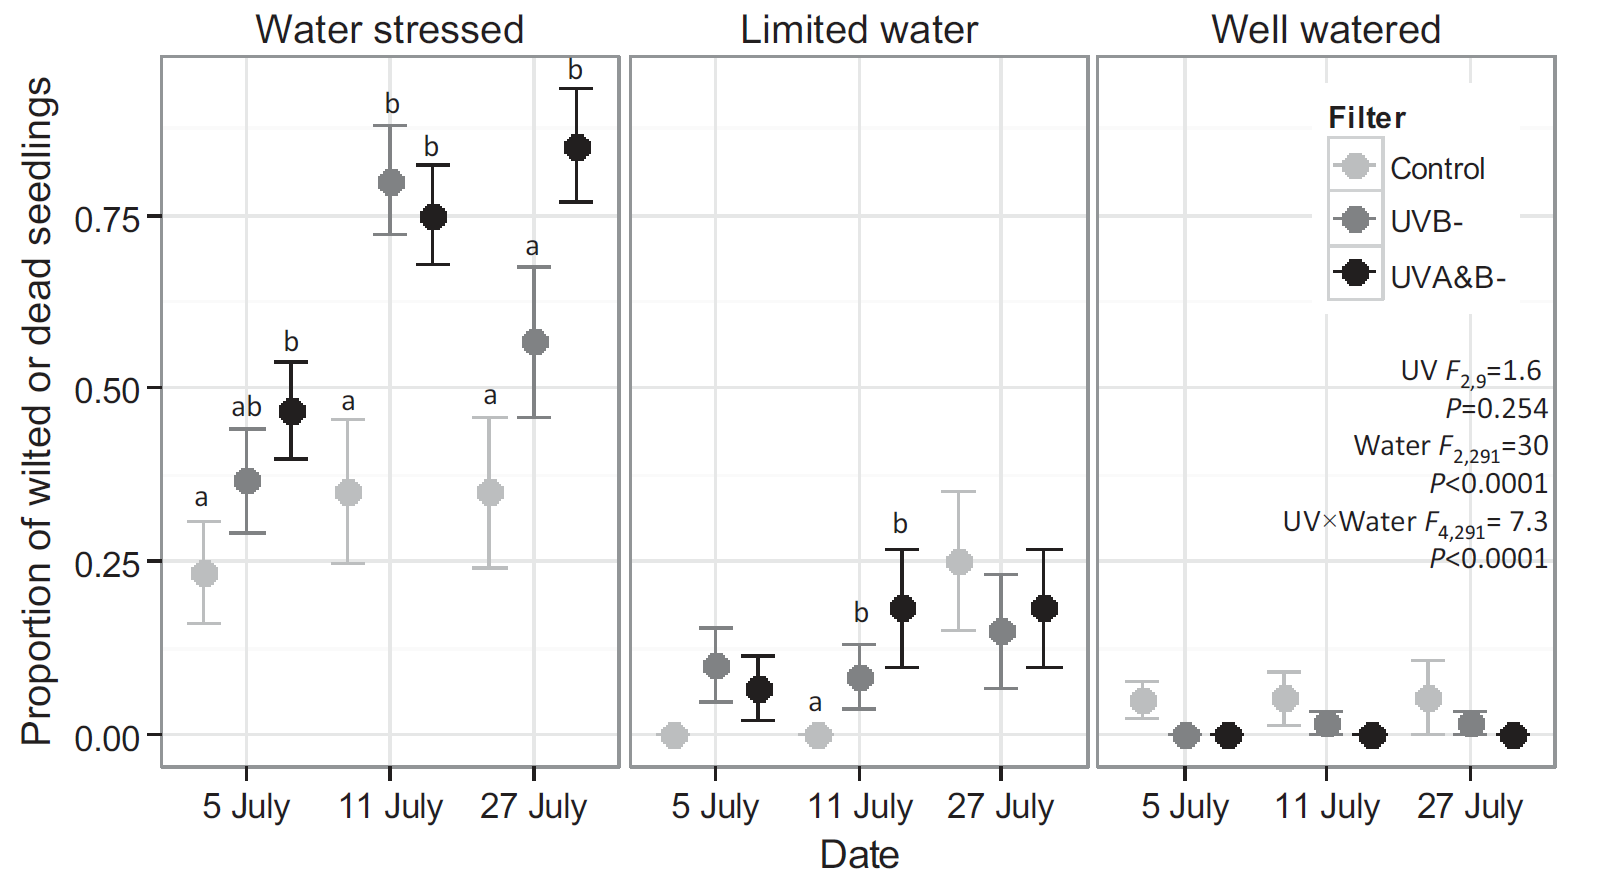
\includegraphics[width=\linewidth]{figures/birch-wilt.png}

  \autocite{Robson2014}
\end{frame}

\begin{frame}[fragile]
  \frametitle{Possible mechanisms: morphology? Yes or No}
\begin{knitrout}\scriptsize
\definecolor{shadecolor}{rgb}{0.969, 0.969, 0.969}\color{fgcolor}

{\centering 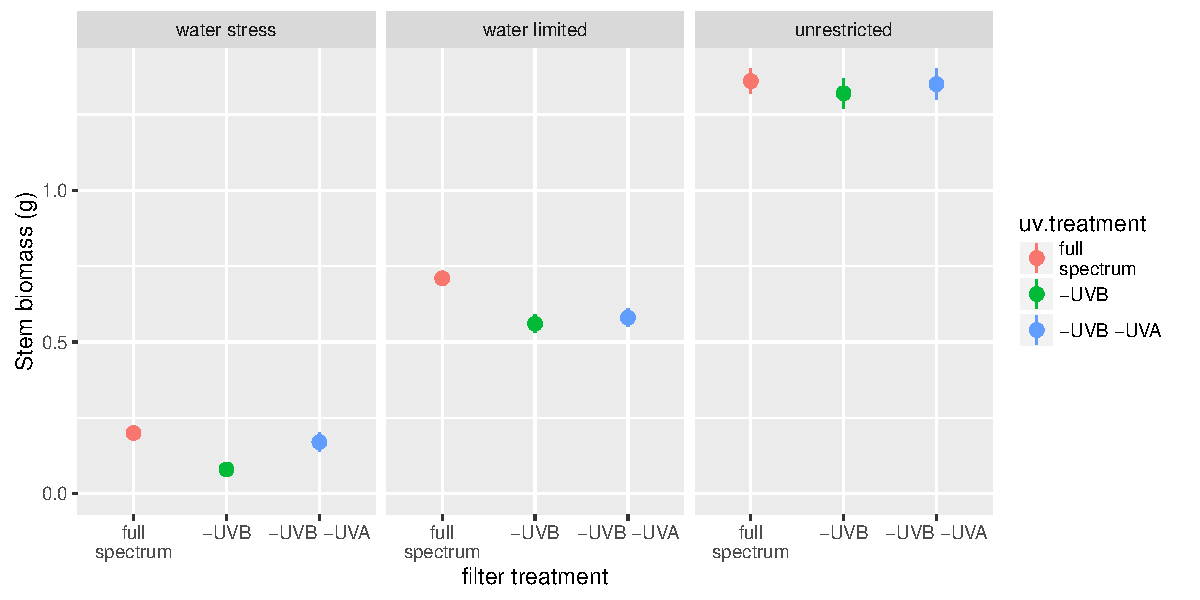
\includegraphics[width=.95\textwidth]{figure/pos-biomass-1} 

}



\end{knitrout}
\end{frame}

%\begin{frame}
%  \frametitle{Possible mechanisms: tissue water relations}
%
%\end{frame}

\begin{frame}[fragile]
  \frametitle{Possible mechanisms: stomatal conductance}
\begin{knitrout}\scriptsize
\definecolor{shadecolor}{rgb}{0.969, 0.969, 0.969}\color{fgcolor}

{\centering 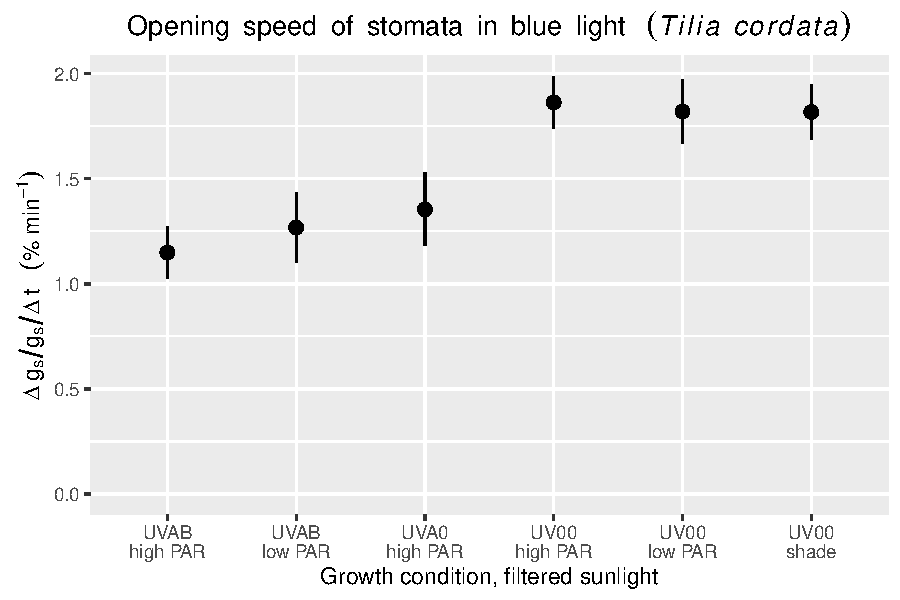
\includegraphics[width=.8\textwidth]{figure/pos-unnamed-chunk-1-1} 

}



\end{knitrout}

(K. Aasamaa and P. J. Aphalo, unpublished)
\end{frame}

%\begin{frame}[fragile]
%  \frametitle{Possible mechanisms: stomatal conductance}
%<<echo=FALSE,fig.width=6, fig.height=4, out.width='.8\\textwidth'>>=
%load(file = "gs_light_summ.rda")
%ggplot(subset(gs_light_summ.df, blue != 0 & green == 0),
%         aes(treatment, gs_rate_mn * 60)) +
%  stat_summary(fun.data = "mean_se") + ylim(0, NA) +
%  labs(x = "Growth condition, filtered sunlight",
%       y = expression(Delta~g[s]/g[s]/Delta~t~~~("%"~min^{-1}))) +
%  ggtitle(expression(Opening~~speed~~of~~stomata~~"in"~~blue~~light~~~(italic(Tilia~~cordata))))
%@
%
%\autocite{Aasamaa2016}
%\end{frame}

\begin{frame}
  \frametitle{Possible mechanisms: gene expression}
  \begin{itemize}
    \item RNAseq + Gene Ontology analysis
       \begin{itemize}
         \item Working on this (tried AgriGo, starting with Bioconductor topGO now)
       \end{itemize}
    \item RNAseq + KEGG pathway analysis
       \begin{itemize}
         \item Bioconductor edgeR and topKEGG
         \item Please see Neha Rai et al.'s poster.
       \end{itemize}
   \item Earlier observations on effects of UVB on genes related to
      \begin{itemize}
        \item phenolic metabolism
        \item ABA signalling
        \item energy metabolism
        \item photosynthesis
        \item cell growth
      \end{itemize}
  \end{itemize}
\end{frame}

\section{Preemptive acclimation: implications}

\begin{frame}
  \frametitle{Take home message}
  If our hypothesis holds for a wide range of species
  \begin{itemize}
    \item reduced growth under UV-B exposure could improve fitness instead of being deleterious,
    \item phenotyping for drought tolerance in dryland crops in the absence of UV-B could lead to little progress,
    \item what should we do with field crops under irrigation: do we need to breed out some of the UVB responses?,
    \item what about rain shelter experiments: should we supplement with UVB?
    \item What about climate change: should we acknowledge that changes in rainfall will correlate with changes in UVB?
  \end{itemize}
\end{frame}

\begin{frame}[<+->]
  \frametitle{Teaser: can you guess how long ago has this text been published?}
\begin{quotation}
\ldots the beneficial effects of ultraviolet
on the animal organism have, in recent years, encouraged the
attempt to demonstrate similar effects on plants, with the result that
a great number of short experiments have been reported in which the
lack of adequate controls has rendered the conclusions of doubtful
value.

\ldots\pause

  The interest in
ultra-violet in recent years has been so widespread as to justify the
accusation of some that the subject is a fad. It is to be hoped that the
"fad" will not run its course before accurate information has been
obtained.
\end{quotation}
\pause
\autocite{Popp1936}
\end{frame}


\section{Acknowledgements}

\begin{frame}[t]
\begin{small}
\begin{tabular}{cp{0.7\textwidth}}
\href{http://blogs.helsinki.fi/senpep-blog/}{\pgfuseimage{SenPEP}} & Members of my research group: Luis O. Morales, Fang Wang, Neha Rai, Yan Yan, Krõõt Aasamaa.\\
                                                                    & Collaborators: T. Matthew Robson, Anders Lindfors, \mbox{Víctor} Sadras, Jorge J. Casal, Saara Hartikainen, David Israel\\

\href{http://blogs.helsinki.fi/vips-blog/}{\pgfuseimage{ViPS}} & A new umbrella organization at our campus.\\

\href{http://www.helsinki.fi/en/}{\pgfuseimage{HYflame}} & My employer.\\

\href{http://www.aka.fi/en/}{\pgfuseimage{AKA}} & For funding, decisions 252548, 16775.\\

\href{http://www.metsatieteellinenseura.fi/english}{\pgfuseimage{SMS}} & For a travel grant to me to come to Pécs.\\

\href{http://www.photobiology.eu/}{\pgfuseimage{ESP}} & For a travel grant to Yan Yan to come to Pécs.\\

\end{tabular}
\end{small}

\end{frame}

\begin{frame}[allowframebreaks,t]
\printbibliography
\end{frame}

\end{document}

